\section{Graphical user interface (GUI)}

\begin{figure}
   \centering
   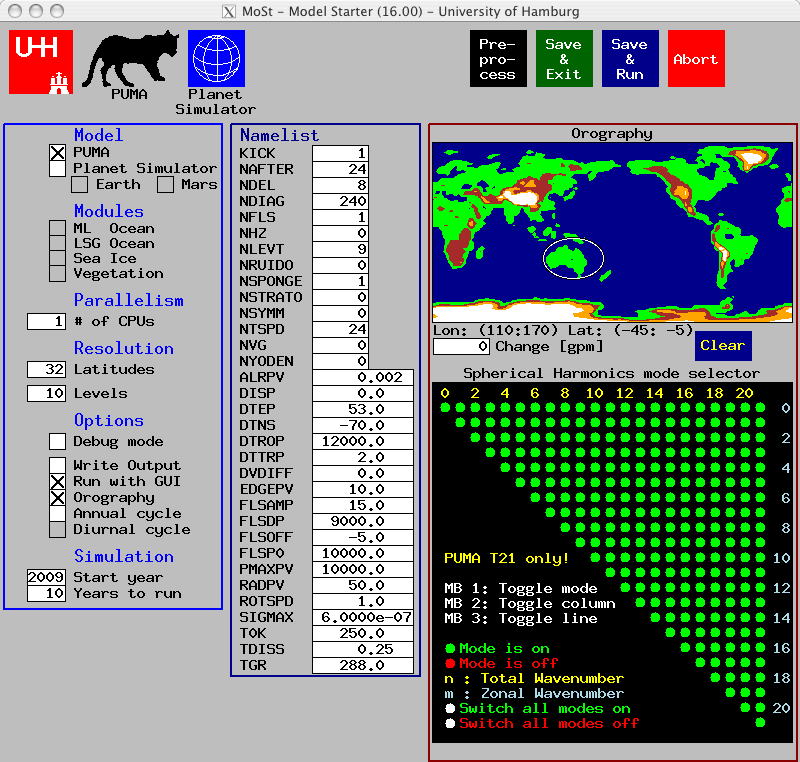
\includegraphics[width=14cm]{Pics/mostsnap}
   \caption[]{Screenshot of Model Starter (MoSt)}
   \label{mostsnap}
\end{figure}

{\bf PUMA} may be used in the traditional fashion,
with shell scripts, batch jobs, and network queuing 
systems. This is useful for long running simulations
on complex machines and number crunchers, such as vector 
computers, massive parallel computers and workstation clusters.
However, there is now a more convenient method.
A graphical user interface (GUI) has been provided, which 
can be used for parameter configuration during model setup, and 
for interaction between the user and the model.


PUMA is setup and configured using the first
GUI module named {\module MoSt} ({\bf Mo}del {\bf St}arter, 
screenshot in \ref{mostsnap}). 
{\module MoSt} is the fastest way to get the
model running. It gives access to the most important parameters of
the model which are preset to the frequently used values.
The model can be started with a mouse click on the button
labelled ``Save \& Run'' either with the standard parameter setting,
or after editing the parameters in the MoSt window.
Some parameters, like horizontal and vertical resolution
or the number of processors, require that a new executable is built
(compile, link and load). MoSt achieves
this by generating and executing build scripts,
that perform the necessary code changes and
create the required executables.
Other parameters defining startup and
boundary conditions or other settings, can
be edited with MoSt. After they have been checked for
correct range and for consistency with other parameters, they
are written to the model's namelist file.

Using these settings
MoSt generates a run script for the simulation.
The user then has the choice of leaving MoSt and
starting the simulation under the control of the GUI
immediately, or of leaving MoSt with the scripts ready
to run. This second alternative is useful for users who
want to include setup modifications beyond the scope of MoSt,
or who want to run the model without the GUI.

There is also a simple graphical editor for the topography.
Check the box Orography and then use the mouse to mark
elliptic areas in the topographic display.
Enter a value for raising (positive) or lowering (negative) the area
and press the button labelled {\bf Preprocess}.
The preprocessor will be built and executed, and a new
topography will be computed and written to the start file.

Another editor is the Mode Editor for spherical harmonics.
Green modes are enabled, red modes are disabled.
This feature can be used to specify runs with only certain
modes of spherical harmonics being active.
LMB, MMB and RMB refer to the left, middle, and right mouse
buttons respectively. You may toggle individual modes (press LMB)
or whole lines (press RMB) and columns (press MMB). 
Currently the Mode Editor can only be used
for PUMA in the T21 resolution.

\begin{figure}
   \centering
   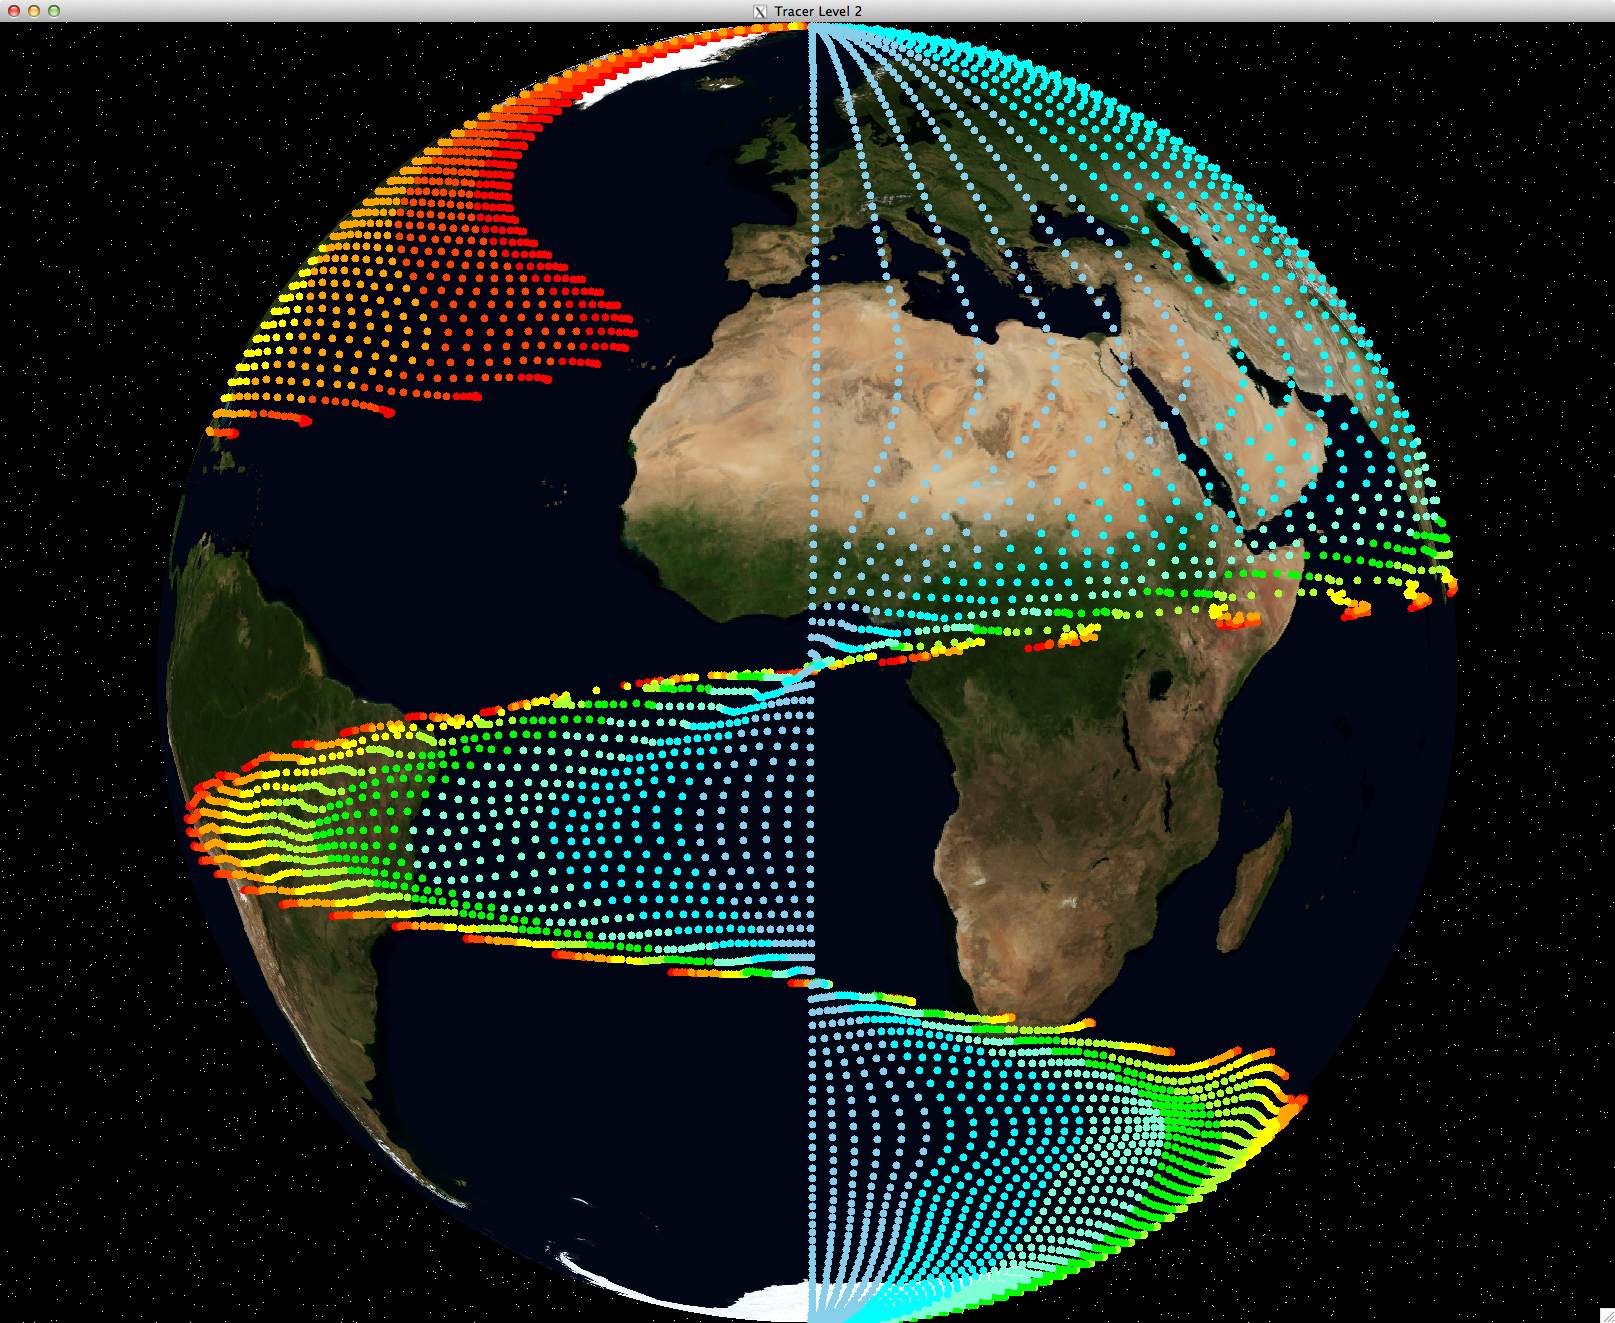
\includegraphics[width=14cm]{Pics/guisnap}
   \caption[]{Screenshot of Graphical User Interface (GUI)}
   \label{guisnap}
\end{figure}

The GUI for running PUMA
(Figure \ref{guisnap})
has two main uses. The first is to display the
model arrays in suitable representations.
Current implementations are:
\begin{itemize}
\item{Zonal mean cross sections}
\item{Horizontal global fields in cylinder or polar projection}
\item{Horizontal particle tracer in cylinder or polar projection}
\item{Longitude-time (Hovmoeller) diagrams}
\item{Longitude-level diagrams}
\item{Amplitudes of spherical harmonic coefficients}
\item{Time series}
\item{Numerical values}
\end{itemize}

In the case of horizontal global grids, pressing the MMB 
toggles between cylinder and polar projection. If the grid is
a single level of a three dimensional field like u or v,
the level being shown can be decreased with the LMB or increased with the RMB.
For Hovmoeller and longitude height sections the LMB and RMB can
be used to select the latitude.

The second use of the GUI is to allow the user to change
selected model variables during the model run.
It is not necessary, though possible, to pause the
model while changing variables. Changes to model variables
are written to the output file after being checked
by the GUI for the appropriate range of values and the 
maximum possible change per timestep, because 
a rapid parameter change or a choice of values beyond the normal
range may cause the model to crash.

All model variables, which are candidates for display
or for interactive changes, have special code to communicate
with PUMA. The experienced modeller
can add new code for additional variables using the existing
communication code as a template. Thus all model fields
or even fields received via coupling with other models
can be shown on the GUI display.

Both, MoSt and the GUI are implemented using Xlib (X11R5),
which is a library of routines for graphics and event communication.
As this library is part of every UNIX/Linux operating system
and is the base of all desktop environments, there is no need
to install additional software for running MoSt and the GUI.
Another important  property of Xlib is full network transparency.
The display of MoSt and the GUI is not confined to the machines
running the programs or the model. In fact, the best
performance is obtained by running the PUMA on
two or four CPUs of remote servers while displaying
the GUI on the user's workstation.
In summary, MoSt and the GUI programs automate many tedious tasks,
minimize the time to become familiar with the PUMA,
and make debugging and parameter tuning much easier.
More types of presentation, coordinate projections
and interactivity are being developed.
A graphical preprocessor with editor for boundary
conditions and a graphical postprocessor are part of the planned
future expansion
to build an almost complete environment for modellers.

\section{GUI configuration}

On initialization, the GUI reads its configuration from a file called
{\bf GUI.cfg} which must be present in the current directory.
MoSt copies the file {\bf GUI.cfg} from the ../dat/ directory
to the run directory while building PUMA.
After reading {\bf GUI.cfg} an attempt is made to read the file
{\bf GUI\_last\_used.cfg}. This file is always written at the end
of a GUI controlled simulation. So one may rearrange and position
GUI windows during a run and the new layout will be saved to the
file {\bf GUI\_last\_used.cfg}. In order to make this user
layout the default for te following runs, just copy this file:
\begin{verbatim}
Most15/puma/run$ cp ../dat/GUI.cfg ../dat/GUI.cfg.old
Most15/puma/run$ cp GUI_last_used.cfg ../dat/GUI.cfg
\end{verbatim}
MoSt will then copy your new layout to the run directory at 
the next invocation.

The {\bf GUI.cfg} is a text file that may also be edited manually.
There is a section for each window (counting from 0 to 8) which
looks like:

\begin{verbatim}
[Window 00]                       <- window number (0..8)
Array:CSU                         <- array name
Plot:ISOCS                        <- picture type
Palette:U                         <- colour palette
Title:Zonal Wind [m/s]            <- window title
Geometry:  529  299    2    3     <- width height left top

[Window 01]
Array:SPAN
Plot:ISOSH
Palette:AMPLI
Title:Spherical Harmonics Ps
Geometry:  529  299  535    3

...

\end{verbatim}

Possible values for these items are:

\subsection{Array}
\begin{tabular}{|l|l|}
\hline
Name     & Description \\
\hline
CSU      & Cross Section U - Zonal mean zonal wind \\
CSV      & Cross Section V - Zonal mean meridional wind \\
CST      & Cross Section T - Zonal mean temperature \\
SPAN     & Spherical harmonic coefficients of surface pressure \\
GU       & Three dimensional grid of zonal wind \\
GV       & Three dimensional grid of meridional wind \\
GP       & Grid of surface pressure \\
SCALAR   & Selected scalars for time series and tables \\
\hline
\end{tabular}

\subsection{Plot}
\begin{tabular}{|l|l|}
\hline
Name     & Description \\
\hline
   ISOHOR & Isolines and colouring of horizontal grids \\
   ISOCS &  Isolines and colouring of cross sections \\
   ISOHOV & Colouring of Hovmoeller diagram \\
   ISOTS &  Timeseries \\
   ISOTAB & Tables \\
   ISOSH &  Coloured amplitudes \\
   ISOLON & Isolines and colouring of longitude height section \\
   ISOTRA & Show the horizontal wind components with moving particles \\
\hline
\end{tabular}

\subsection{Palette}
\begin{tabular}{|l|l|l|}
\hline
Name     & Range & Description  \\
\hline
   AUTO & automatic & rainbow colours \\
   U &    -10 .. 50 & rainbow colours \\
   V &    -10 .. 10 & rainbow colours \\
   T &    -50 .. 50 & blue - red \\
   P &    985 .. 1025 & blue - red \\ 
   Q &      0 .. 60 & rainbow colours \\
   MARST & -90 .. 0 & blue -red \\
   AMPLI & 0 .. 12 & blue - green -red \\
   VEG   & 0 .. 100 & shades of green \\
\hline
\end{tabular}

\subsection{Title}
The title item may contain any text, but keep it short.
The length of the window's title bar is limited.
The words {\em Latitude} and {\em Level} have special
features in conjunction with three-dimensional arrays,
where the user may scroll the level or latitude.
The GUI will insert the level number after the word 
{\em Level} or the latitude after the word {\em Latitude}.

\subsection{Geometry}
The four integers following the geometry item describe
the size and screen position of the window.
The first two parameters refer to width and height in 
screen pixels. These are the sizes of the inner window.
The title bar, the border and any other decorations are not counted.
The third and fourth parameter set the x and y coordinates of the
upper left corner of the window, again without borders.
If the geometry item is not defined, the GUI will
initialize the window's geometry depending on the screen size.


